\section{A type system for determinism}\label{design}

This section presents the key aspects of our type system
% , called \ourTypeSystem,
in the context of a core calculus for an
object-oriented language.


\subsection{Preliminaries and notation}

%% This section is too basic, and therefore is boring because most readers
%% will already know it.  It also delays the interesting parts of the paper
%% for too long.  We can introduce concepts as they are needed in the rest
%% of the paper.
% \subsection{Type checking background}\label{type-checking}
% The major components of a type system include: 1) \textit{types}, 2) \textit{subtyping rules}, and 3) \textit{dataflow analysis}.
% A \textit{type} serves as an abstraction for the set of acceptable values for any expression. The types in a type system form a lattice of finite height. 
% The hierarchy of types in this lattice defines subtyping relationships among them.
% In our framework, we require every type hierarchy to define a unique\<@Top> and a \<@Bottom> element. This ensures that
% any given pair of types has a \textit{least upper bound} and a \textit{greatest lower bound}.
% Throughout this paper, we use the notation \<@A> <: \<@B> to denote that type \<@A> is a subtype of type \<@B>.
% As an illustration of the type hierarchy, consider the lattice of types shown in \cref{fig-example-lattice}.
% \begin{figure}
%     \begin{center}
%         \includegraphics[scale=0.15]{lattice}
%     \end{center}
%     \caption{Example type hierarchy}
%     \label{fig-example-lattice}
% \end{figure}
% In this type system, \<@C> is a subtype of \<@A> as well as \<@B> and types \<@A> and \<@B> are incomparable.
% The type checker now performs additional type checking (similar to javac's type checking) with respect to this type hierarchy
% and reports any violations. The snippet in \cref{code-invalid1} would result in an error at the assignment statements:
% \begin{figure}
%     \begin{verbatim}
%     @A int x; @B int y; @C int z;
%     x = y;    // Because types @A and @B are incomparable.
%     z = x;    // Because @C is a subtype of @A.
%     \end{verbatim}
% \caption{Example: Invalid assignment}
% \label{code-invalid1}
% \end{figure}
% 
% %Method overriding and example
% For method overriding, the usual rules apply for parameters and arguments i.e covariant subtyping for parameters
% and contravariant subtyping for return types. Consider the example in \cref{code-invalid2} where method \<foo> of \<class X> is overridden
% in \<class Y>.
% \begin{figure}
%     \begin{verbatim}
%     class X {
%         @B int foo(@C int param) {}
%     }
%     class Y extends X {
%         @C int foo(@B int param) {}
%     }
%     \end{verbatim}
%     \caption{Example: Invalid Method override}
%     \label{code-invalid2}
% \end{figure}
% 
% The overriding method is invalid for two reasons: type of the parameter (\<@B>) is not a subtype of the parameter type in the overridden method (\<@C>) and the return type (\<@C>) is not a supertype of the return type of the overridden method (\<@B>).
% 
% %collections type parameters - invariant
% Collection types are invariant. So, if a \<List> x is declared as \codeid{@A List<@A String> x;} and another \<List y> is declared
% as  \codeid{@A List<@B String> y;}, writing \<x = y> would result in an error.
% 
% %covariant array types
% Arrays follow covariant subtyping rules in java. Therefore, the assignment statement \<@A int @A[] x = y;> where \<y> was 
% declared as \<@B int @A[] y> would type check without any warning.



%\todo{Need some background around here about what a type qualifier is,
%  how it is represented in Java, and how to read a type \<@Q BaseType>.}

%\todo{Greek letters go after this paragraph.}

\begin{figure}
  \newcommand{\bnfalt}{\ \ |\ \ }
  \begin{tabular}{lcll}
    $C$ & ::= & \<Int>\bnfalt \<String>\bnfalt \<Collection>\bnfalt \<List>\bnfalt \<Set>\bnfalt \<Map> & class name \\
    $\kappa$ & ::= & \<NonDet>\bnfalt \<OrderNonDet>\bnfalt\<Det> & type qualifier \\
    $\tau$ & ::= & $\kappa\ \beta$ & \mbox{type} \\
    $\beta$ & ::= & $C$\bnfalt $C\angles{\overline{\tau}}$ 
    & \mbox{unqualified type}
  \end{tabular}
  \caption{Grammar of types}
  \label{fig:grammar}
\end{figure}

One way to view a type is as
a set of values.  A type abstracts or restricts the
set of possible run-time values that an expression may evaluate to
and the operations that may be performed.
A programming language provides \emph{basetypes}, such as \<Int>.
A \textit{type qualifier} on a basetype adds additional constraints;
that is, it reduces the size of the set of values.
An example type qualifier is \<Positive>, and a type (which combines a qualifier
and a basetype) is \<Positive Int>.
A polymorphic type abstraction such as \<List> can be instantiated by a type argument,
as in \ptype{List}{Positive Int}.

\Cref{fig:grammar} formalizes these notions.
For simplicity of exposition,
\cref{fig:grammar}'s $\beta$ is not a basetype as described above:  $\beta$
lacks a top-level type, but any type arguments are full types
$\tau$.
In our core calculus, a type $\tau$ always has a qualifier.
Our implementation, \theDeterminismChecker, uses inference (\cref{sec:dataflow-java}) and
defaults (\cref{defaulting}) to
permit users to omit type qualifiers.


A type checker verifies the types written in a program.
\OurTypeSystem checks all the standard typing rules including the ones
shown in \cref{typecheck-rules-standard}, which
shows a sample of standard typing rules for
an object-oriented programming language.
% For \ourTypeSystem, $\tau$
% represents a qualified type rather than a basetype.

A type qualifier constrains the set of possible run-time values, that is,
$\kappa \ \beta \sqsubseteq \beta$.
As a result, a qualifier type system does not allow any values that the
original type system does not, in the same program without qualifiers.
However, the qualifier type system may reject more programs, and thus
affords stronger guarantees.
% (Our implementation \theDeterminismChecker runs the underlying base type
% system, then issues additional errors and warnings.)

Type qualifier systems are sometimes defined independently of the
underlying type system.  In \ourTypeSystem, there are interactions between the
basetypes and the type qualifiers.  Defining them together improves
precision, which is important in practice.


\begin{figure}
    \bigskip

    $\infer{\tau_1 \sqsubseteq \tau_3}{\tau_1 \sqsubseteq \tau_2 \quad \tau_2 \sqsubseteq \tau_3}
    \quad\quad
    \infer[\rulename{subtyping}]{\Gamma \vdash x : \tau_2}{\Gamma \vdash x : \tau_1 & \tau_1 \sqsubseteq \tau_2}$
    
    \bigskip
    
    $\infer[\rulename{call}]{\Gamma \vdash f(\overline{a_i}) : \tau_r}
    {\Gamma \vdash f : \overline{\tau_i} \rightarrow \tau_r & \Gamma \vdash \overline{a_i : \tau_i}}$
    
    \bigskip
    
    $\infer[\rulename{invariant type arg}]{C_1\angles{\overline{\tau_i}}
      \sqsubseteq C_2\angles{\overline{\tau_i}}}{C_1 \sqsubseteq C_2}$
    
    \caption{A sampling of standard typing rules.  We omit other standard rules,
    for brevity.}
    \label{typecheck-rules-standard}
\end{figure}

\begin{figure}
    \bigskip

    $\infer{\Det \sqsubseteq \OrderNonDet}{}
    \quad\quad
    \infer{\OrderNonDet \sqsubseteq \NonDet}{}$
    
    \bigskip

    $\infer{\kappa_1 \beta \sqsubseteq \kappa_2 \beta}{\kappa_1 \sqsubseteq \kappa_2}
    \quad\quad
    \infer{\kappa\ \beta_1 \sqsubseteq \kappa\ \beta_2}{\beta_1 \sqsubseteq \beta_2}$
    
    
    \caption{Subtyping rules for \ourTypeSystem's type qualifiers.  $\sqsubseteq$ is overloaded for classes,
    type qualifiers, types, and unqualified types $\beta$.}
    \label{fig:typecheck-rules}
\end{figure}


%\todo{Define the Greek.  For example:
%
%  A type $\tau = \kappa\ \beta$ consists of a qualifier and a basetype.
%  Neither may be omitted.
%
%  $\beta$ is a type that lacks its type qualifier, but has type qualifiers
%  on any type arguments:
%  $\beta = C | C\angles{\overline{\tau}}$.
%  }




\subsection{Determinism types}\label{type-hierarchy}

%% Reinstate wrapfigure later.  But, if it spans pages, every following
%% page to the end of the document is narrowed to accommodate it.
% \begin{wrapfigure}{R}{0.3\textwidth}
\begin{figure}
    \begin{center}
        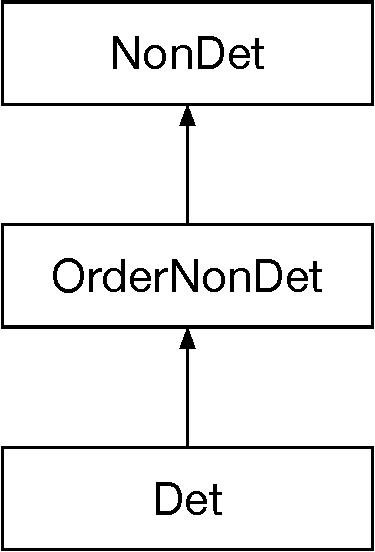
\includegraphics[scale=0.37]{detHierarchy}
    \end{center}
    \caption{Determinism type qualifier hierarchy}
    \label{fig:determinism-hierarchy}
\end{figure}
% \end{wrapfigure}

The core of the determinism type system is the following type qualifiers:
\begin{itemize}
    \item \<NonDet> indicates
    that the expression might have different values in two different executions.
    \item \<OrderNonDet> indicates that the expression is a collection or
      map that contains the same elements in every execution, but possibly
      in a different order.
    \item \<Det> indicates that the expression evaluates to equal values in
      all executions; for a collection, iteration
      also yields the values in the same order.
\end{itemize}
\Cref{fig:typecheck-rules,fig:determinism-hierarchy} show the subtyping
relationship among the qualifiers.

\<OrderNonDet> may only be written on collections and maps.
A map is a dictionary or an associative array, such as a hash table.
\OurTypeSystem largely treats a map as a collection of key--value pairs.
Both collections and maps may be \<Det>, \<OrderNonDet>, or \<NonDet>.
The basetypes of their elements can be specified independently of the collection basetypes.
However, an element type qualifier must be a subtype of the collection type qualifier.
The next section discusses type well-formedness in detail.
%and
%the element types can be specified independently of the collection type,
%including their qualifiers.

%\todo{A type $\tau$ is represented as $\kappa \ \beta$
%where $\kappa$ is a type qualifier (that is, \<NonDet>, \<OrderNonDet>, or
%\<Det>) and $\beta$ is a Java basetype.}


\subsection{Collection types}\label{collection-rules}

\subsubsection{Type well-formedness}

%\todo{Note that the \rulename{ordernondet} versions also handle \<Det>,
%  because $\<Det> \sqsubseteq \<OrderNonDet>$.}

\begin{figure}
    $\infer[\rulename{noncollection}]
    {\wellformed{\kappa \  \beta}}
    {\kappa \in \{ \<Det>, \<NonDet> \} & \beta \not\sqsubseteq \<Collection> & \beta \not\sqsubseteq \<Map>}$
    
    \bigskip
    
    $\infer[\rulename{ordernondet collection}]
    {\wellformed{\kappa_c \  C \angles{\kappa_e \ \beta_e}}}
    {\kappa_c \sqsubseteq \<OrderNonDet> &
      C \sqsubseteq \<Collection> &
      \kappa_e \sqsubseteq \kappa_c &
      \wellformed{\kappa_e \ \beta_e}}$
    
    \bigskip
    
    $\infer[\rulename{nondet collection}]
    {\wellformed{\<NonDet> \ C\angles{\<NonDet> \ \beta_e}}}
    {C \sqsubseteq \<Collection> & \wellformed{\<NonDet> \ \beta_e}}$
    
    \bigskip
    
%      $\infer[\rulename{ordernondet array}]{\wellformed{\kappa_e \ \beta_e \ \  \kappa_a []}}{\kappa_a \sqsubseteq \<OrderNonDet> & \kappa_e \sqsubseteq \kappa_a }$
%     
%     \bigskip
%     
%     $\infer[\rulename{nondet array}]{\wellformed{\<NonDet> \ \beta_e \ \  \<NonDet> []}}{}$
%     
%     \bigskip
    
    $\infer[\rulename{ordernondet map}]
    {\wellformed{\kappa_m \  C \angles{\kappa_k \ \beta_k, \kappa_v \ \beta_v}}}
    {\kappa_m \sqsubseteq \<OrderNonDet>
      & C \sqsubseteq \<Map>
      & \kappa_k \sqsubseteq \kappa_m
      & \kappa_v \sqsubseteq \kappa_m
      & \wellformed{\kappa_k \ \beta_k}
      & \wellformed{\kappa_v \ \beta_v}
    }$
    
    \bigskip
    
    $\infer[\rulename{nondet map}]
    {\wellformed{\<NonDet> \ C\angles{\<NonDet> \ \beta_k, \<NonDet> \ \beta_v}}}
    {C \sqsubseteq \<Map> & \wellformed{\<NonDet> \ \beta_k} & \wellformed{\<NonDet> \ \beta_v}}$
    
    \caption{Type well-formedness}

%\todo{\todo{I think this will be OK, by redefining $\beta$.}
%  The collection rules do not permit nested collections; similarly, the
%  (currently commented out) array rules did not permit any two-dimensional
%  array to be well-formed.  There is a bigger issue here.
%  Consider the ``nondet collection'' rule.  $C_c$ is a class (we need
%  to use a different symbol for it, probably $c$), but $\beta_e$ should be
%  a full type, which might contain type qualifiers within it.  (Actually,
%  $\<NonDet>\ \beta_e$ is a type, not $\beta_e$ itself.)  So, there should
%  be an antecedent stating that $\<NonDet> \beta_e$ is well-formed, and
%  for the ``ordernondet collection'' rule stating that $\kappa_e \beta_e$
%  is well-formed.  Likewise, antecedents are needed for the map rules.
%  Otherwise, these rules permit construction of $\<Map>\angles{\tau'}$
%  where $\tau'$ is itself not well-defined.}

  \label{type-validity}
\end{figure}

% "invalid" is easier to read than "non-well-formed".
\Cref{type-validity} shows the type well-formedness, or type validity,
rules of \ourTypeSystem. 

\begin{figure}
    \centering
    \begin{tabular}{|l|l|l|l|l|}
        \cline{3-5}
        \multicolumn{2}{c|}{~}  &  \multicolumn{3}{c|}{Element type} \\ \cline{3-5}
        \multicolumn{2}{c|}{~}  & \<NonDet>     & \<OrderNonDet> & \<Det> \\ \hline
                        & \<NonDet>      &  valid     &  invalid    & invalid  \\ \cline{2-5}
        Collection type & \<OrderNonDet> &  invalid   &  valid      & valid    \\ \cline{2-5}
                        & \<Det>         &  invalid   &  invalid    & valid    \\ \hline
    \end{tabular}
    \caption{Valid Collection declarations.  The Collection's type qualifier
        must be a supertype or equal to the element type.}
    \label{fig:determinism-collections}
\end{figure}

The element type of a \<NonDet> collection must be \<NonDet>.
For other collections, the type qualifier on a collection's element must be a subtype or equal to
the collection's type qualifier (\rulename{collection} rules of
\cref{type-validity}). Note that the \rulename{ordernondet} rules also
permit \<Det> collections,
because $\<Det> \sqsubseteq \<OrderNonDet>$.
\Cref{fig:determinism-collections} restates the \rulename{collection} rules
of
\cref{type-validity}.

\smallskip
\noindent
\begin{minipage}{.48\textwidth}
Some examples of valid types are:
% Using "~" instead of "\ " does not work within \codeid :-(
\begin{Verbatim}[commandchars=\\\{\}]
NonDet      \lptype{List}{NonDet      Int}
OrderNonDet \lptype{List}{OrderNonDet \lptype{Set}{...}}
OrderNonDet \lptype{List}{Det         Int}
Det         \lptype{List}{Det         Int}

\end{Verbatim}
\end{minipage}
\hfill
\begin{minipage}{.46\textwidth}
These types are invalid:
\begin{Verbatim}[commandchars=\\\{\}]
NonDet      \lptype{List}{OrderNonDet \lptype{Set}{...}}
NonDet      \lptype{List}{Det         Int}
OrderNonDet \lptype{List}{NonDet      Int}
Det         \lptype{List}{NonDet      Int}
Det         \lptype{List}{OrderNonDet \lptype{Set}{...}}
\end{Verbatim}
\end{minipage}
\smallskip


%It is possible to store an expression of type \<Det> in a \<NonDet>
%collection, but any value retrieved from a \<NonDet> collection has
%type \<NonDet>.

If the type \ptype{NonDet List}{Det String} were
permitted, the following type hole would exist:

\begin{Verbatim}[commandchars=\\\{\}]
\lptype{Det    List}{Det String} ddlist
\lptype{NonDet List}{Det String} ndlist = ddlist   // assignment permitted by subtyping rules
NonDet Int ni = ...
ndlist[ni] = "anywhere"
\end{Verbatim}

\noindent
In this code snippet,
the deterministic string \<"anywhere"> is placed in the list at an
arbitrary (that is, nondeterministic) index.  This must be prohibited,
because it unsoundly permits the deterministic list \<ddlist> to differ
from execution to execution.  \OurTypeSystem does so by forbidding the type
\ptype{NonDet List}{Det String}.


\subsubsection{Behavior of order-nondeterministic collections}\label{sec:ond-behavior}

A collection of type \<OrderNonDet> has special properties, including the following.

\begin{enumerate}
\item
The individual elements retrieved from it have type \<NonDet>.  This
affects access, iteration, searching, etc.
(As shown by types of methods \rulename{get}, \rulename{iterator}, \rulename{next} in \cref{fig-ordernondet-rules})
\item
Size-related operations return a deterministic result.  This also affects
queries of whether an iterator has more elements.
\item
If the collection is sorted, or its elements are placed in a collection
that does sorting, the result is deterministic.
\end{enumerate}

To state the first point more formally, the 
typical type for a list access operation, such as \<get>, is
$$\forallt{\tau} \<List>\angles{\tau} \times \<Int> \rightarrow \tau$$
but this type is incorrect for \ourTypeSystem.  Each of the following is a
correct (but overly restrictive) type for \<get>:
\begin{eqnarray*}
\forallt{\kappa\ \beta} \<NonDet>\ \<List>\angles{\kappa\ \beta} \times \<Det Int>
& \strut\hspace{-1em} \rightarrow \<NonDet>\ \beta
& \mbox{\quad in this case $\kappa = \<NonDet>$} \\
\forallt{\kappa\ \beta} \<OrderNonDet>\ \<List>\angles{\kappa\ \beta} \times \<Det Int>
& \strut\hspace{-1em} \rightarrow \<NonDet>\ \beta
& \mbox{\quad in this case $\kappa \in \{ \<OrderNonDet>, \<Det> \} $} \\
\forallt{\kappa\ \beta} \<Det>\ \<List>\angles{\kappa\ \beta} \times \<Det Int>
& \strut\hspace{-1em} \rightarrow \<Det>\ \beta\phantom{\<Non>}
& \mbox{\quad in this case $\kappa = \<Det>$}
\end{eqnarray*}

\noindent
and no type introduced so far can express this polymorphism.
(The typing is actually even more complex, because if \emph{either}
argument to \<get> is \<OrderNonDet> or \<NonDet>, then the
result is \<NonDet>.  The above examples only show the case where the index
is deterministic.)
The typical type for the list access operation only applies if both
arguments are \<Det>,
and our typing must have that as a special case, which is the last line above.






\begin{figure}

%    $\infer[\rulename{iteration}]
%    {\Gamma \vdash \|y| : \|OrderNonDet\ Iterator|\angles{\tau}}
%    {\Gamma \vdash \|x| : \|OrderNonDet \ C\angles{\tau}|
%    & C \sqsubseteq \|Collection|
%    & \|y = C.iterator()|
%    & \wellformed{\tau}
%    }$

    \rulename{get}: 
    $
    \forallt{\tau\ \kappa}
    % Not necessary: invalid instantiantions are not created
    % \in \{\<Det>, \<NonDet>\}\
    \<OrderNonDet> \ C \angles{\tau} \ \times \kappa \ \<Int> \rightarrow 
    \<NonDet> \ \<Int>
    $
    
    \bigskip
    
    \rulename{set}: 
    $
    \forallt{\kappa\ \beta} \ \<OrderNonDet> \ C \angles{\kappa \ \beta} \ \times \<Det> \ \<Int> \times \kappa \ \beta \rightarrow 
    \<NonDet> \ \beta
    $
    
    \bigskip
    
%% We don't need this.  Just leaving it out means the expression has no
%% typing and is therefore invalid.
%     \rulename{set invalid}: 
%     $
%     \forallt{\kappa, \beta} \ \<OrderNonDet> \ C \angles{\kappa \ \beta} \ \times \<NonDet> \ \<Int> \times \kappa \ \beta \rightarrow 
%     \|INVALID|
%     $
    
    \rulename{size}:
    $
    \forallt{\tau} \<OrderNonDet>\ C\angles{\tau} \rightarrow
    \<Det> \ \<int>
    $
   

    \bigskip

    \rulename{iterator}: 
    $
    \forallt{\tau} \<OrderNonDet> \ C \angles{\tau} \rightarrow 
    \<OrderNonDet> \ \<Iterator> \angles{\tau}
    $
    
    \bigskip
    
%    $\infer[\rulename{next element}]
%    {\Gamma \vdash \|z| : \|NonDet \ \beta|}
%    {\Gamma \vdash \|y| : \|OrderNonDet \ Iterator\angles{\kappa \ \beta}|
%        & \|z = y.next()|
%        & \wellformed{\kappa \ \beta}
%    }$

    \rulename{next}:
    $
    \forallt{\kappa\ \beta} \<OrderNonDet>\ \<Iterator>\angles{\kappa \ \beta} \rightarrow
    \<NonDet>\ \beta
    $
    
    \bigskip
    
%    $\infer[\rulename{hasnext element}]
%    {\Gamma \vdash \|z| : \|Det \ boolean|}
%    {\Gamma \vdash \|y| : \|OrderNonDet \ Iterator\angles{\tau}|
%        & \|z = y.hasNext()|
%        & \wellformed{\tau}
%    }$

    \rulename{hasnext}:
    $
    \forallt{\tau} \<OrderNonDet>\ \<Iterator>\angles{\tau} \rightarrow
    \<Det> \ \<boolean>
    $

%    $\infer[\rulename{size}]
%    {\Gamma \vdash \|y| : \|Det \ int|}
%    {\Gamma \vdash \|x| : \|OrderNonDet \ C\angles{\tau}|
%        & C \sqsubseteq \|Collection|
%        & \|y = x.size()|
%        & \wellformed{\tau}
%    }$

\caption{\<OrderNonDet> Collection rules.  $C$ is a collection class.
    These are partial types indicating the methods' behavior on
    \<OrderNonDet> arguments.}
%\todo{These should be method names, not rule names, right?  The figure is
%  just giving the types of methods.}
\label{fig-ordernondet-rules}
\end{figure}

\subsection{Polymorphism}\label{polymorphism}

This section first describes basic polymorphism over type qualifiers and
over basetypes (\cref{sec:basic-polymorphism}).  Then, it describes two
extensions.
One extension resolves \<OrderNonDet> to \<NonDet> or \<Det> where
needed (\cref{polymorphism-up-down}).
The other extension permits use of polymorphic (type) variables without
affecting binding of those variables --- that is, it affects which
instantiation of a (method) abstraction is chosen at a use site
(\cref{bindings-uses}).

%\todo{Can we come up with more examples of interesting functions to
%  describe here?  Or put them in section 3.}


\subsubsection{Qualifier and basetype polymorphism}\label{sec:basic-polymorphism}

\OurTypeSystem supports parametric
polymorphism~\cite{Abadi:1989:FIM:77350.77373,Plotkin:1993:LPP:645891.671433}.
A polymorphic abstraction (a class or method) is written and
typechecked once.
It acts as if it has multiple different types, and each use site is
typechecked using the most specific applicable instantiated
non-polymorphic type.




\OurTypeSystem supports both basetype polymorphism and qualifier polymorphism.
When both are applied, it gives the effect of type polymorphism.

\begin{itemize}
\item
Type polymorphism has the usual semantics.  For example, the type of the
identity function is $\forallt{\tau} \tau \rightarrow \tau$, which can be
equivalently written as
$\forallt{\kappa \ \beta} \kappa \ \beta \rightarrow \kappa \ \beta$.


\item
  Basetype polymorphism lets the basetype vary independently of the
  qualifier, which might be fixed or might be polymorphic.
  An example is a nondeterministic \<choose> function, which might have type

  $\<choose> : \forallt{\beta} \<Set>\angles{\<Det>\ \beta} \rightarrow \<NonDet>\ \beta$

  Basetype polymorphism is rarely used on its own.  Full type polymorphism is more
  common, even if the function type decomposes the type parameter and uses the parts independently,
  as in this more general type for the \<choose> function:

  $\<choose> : \forallt{\kappa\ \beta} \<Set>\angles{\kappa\ \beta} \rightarrow \<NonDet>\ \beta$

\item
Qualifier polymorphism is common.  For example, here are types for
the \<length> method on strings and the addition operation:

$\<length>\ :\ \forallt{\kappa} \kappa\ \<String> \rightarrow \kappa\ \<Int>$

$\<plus>\ :\ \forallt{\kappa} \kappa\ \<Int> \times \kappa\ \<Int> \rightarrow \kappa\ \<Int>$

\end{itemize}

Informally, the \<length> method above acts as if it had multiple
(overloaded) definitions

$\<length>\ : \<NonDet>\ \<String> \rightarrow \<NonDet> \ \<Int>$

$\<length>\ :\<Det>\ \<String> \rightarrow \<Det> \  \<Int>$

\noindent
The body of \<length> must typecheck at every possible instantiation of its
polymorphic function type.  At a use site of \<length>,
the most specific applicable instantiation is chosen.

For example,
suppose we have two variables $\<ni> : \<NonDet Int>$ and $\<di> : \<Det Int>$.
This table shows, for several method invocations, the 
most specific applicable instantiation for that invocation and the type of
the call expression:

\begin{tabular}{lll}
  Expression & instantiation & type \\
\<plus(ni, ni)> & $\<NonDet>\ \<String> \rightarrow \<NonDet> \ \<Int>$ & \<NonDet> \\
\<plus(di, di)> & $\<Det>\ \<String> \rightarrow \<Det> \ \<Int>$ & \<Det> \\
\<plus(ni, di)> & $\<NonDet>\ \<String> \rightarrow \<NonDet> \ \<Int>$ & \<NonDet> \\
\<plus(di, ni)> & $\<NonDet>\ \<String> \rightarrow \<NonDet> \ \<Int>$ & \<NonDet> \\
\end{tabular}

\smallskip

We adopt the convention that  polymorphism is not instantiated in ways
that would create invalid types.  For example, the \<length> and \<plus> polymorphic
functions would not be instantiated at $\kappa = \<OrderNonDet>.$
This makes no difference for these particular functions:  such an
instantiation would never be the most specific applicable one.
The general rule about instantiations and type validity
is important for some of the type rules given in this paper, which
would otherwise need complex preconditions that recapitulate the type
well-formedness rules.


\subsubsection{Polymorphism rules for collections}\label{polymorphism-up-down}

As described so far, polymorphism cannot express the collection behaviors
of \cref{sec:ond-behavior}.
Consider this potential typing for the \<size> method in class \CollectionE:

$\<size>\ :\ \forallt{\kappa} \kappa\ \CollectionE \rightarrow \kappa\ \<Int>$

\noindent
It cannot be instantiated at $\kappa = \<OrderNonDet>$ as 

$\<size>\ :\ \<OrderNonDet>\ \CollectionE \rightarrow \<OrderNonDet>\ \<Int>$

\noindent
because such an instantiation would include the invalid return type \<OrderNonDet Int>.
This means that the only two instantiations are at 
$\kappa = \<NonDet>$ and $\kappa = \<Det>$.  An invocation on an
\<OrderNonDet> collection would choose the \<NonDet> instantiation, and the
return type at that call site would be \<NonDet Int> rather than the
desired \<Det Int>.

\begin{figure}
    $\infer{\up{\<NonDet>} = \<NonDet>}{}
    \quad
    \infer{\up{\<OrderNonDet>} = \<NonDet>}{}
    \quad
    \infer[\rulename{polyup}]{\up{\<Det>} = \<Det>}{}
    $

    \bigskip
    
    $\infer{\down{\<NonDet>} = \<NonDet>}{}
    \quad
    \infer{\down{\<OrderNonDet>} = \<Det>}{}
    \quad
    \infer[\rulename{polydown}]{\down{\<Det>} = \<Det>}{}
    $

\caption{Polymorphic resolution of $\uparrow$ and $\downarrow$ operators.  $\uparrow$ is overloaded for types and qualifiers.}
\label{fig:poly-resolutions}
\end{figure}

\OurTypeSystem resolves this problem by introducing two operators over
polymorhic (type) variables, $\uparrow$ and $\downarrow$.
The $\uparrow$ operator converts \<OrderNonDet> to \<NonDet> and leaves the
other qualifiers unchanged.  The upward-pointing arrow is mnemonic for replacing
\<OrderNonDet> by something higher in the type hierarchy.
The $\downarrow$ operator is analogous, but it converts \<OrderNonDet> to
\<Det>, which is lower in the type hierarchy.
\Cref{fig:poly-resolutions} formalizes their behavior.



% Not true: We allow Poly(up) and down at every location where Poly is allowed.
%Valid locations for \codeid{@PolyDet("up")} and  \codeid{@PolyDet("down")}:
%$\infer{\wellformed{\kappa \  \beta}}{isParam(\beta) / isReturn(\beta) & \kappa : @PolyDet("up") / @PolyDet("down")}$
%
%Resolution of \<@PolyDet("up")>:\todo{typesetting}
%
%$\infer{\Gamma \vdash x : @NonDet \ \beta_a}{\Gamma \vdash x : \kappa_a \ \beta_a &  \kappa_a : @OrderNonDet/@NonDet & \kappa_p : @PolyDet("up") & \kappa_p \ \beta_p : declaration \ type & \kappa_a \ \beta_a : resolved \ type}$
%
%Resolution of \<@PolyDet("down")>:
%
%$\infer{\Gamma \vdash x : @Det \  \beta_a}{\Gamma \vdash x :  \kappa_a \beta_a & \kappa_a : @OrderNonDet/@Det & \kappa_p : @PolyDet("down") & \kappa_p \ \beta_p : declaration \ type & \kappa_a \ \beta_a : resolved \ type}$


%\Cref{fig-poly-resolution} presents the rule for type checking of methods annotated with \<PolyDet> or its variants.

The correct type for \<size> is

$\<size> : \forallt{\kappa} \kappa\ \CollectionE \rightarrow \down{\kappa}\ \<Int>$

\noindent
This can be instantiated at all three type qualifiers without creating any
invalid types:

$\<size> : \<NonDet>\ \CollectionE \rightarrow \<NonDet>\ \<Int>$

$\<size> : \<OrderNonDet>\ \CollectionE \rightarrow \<Det>\ \<Int>$

$\<size> : \<Det>\ \CollectionE \rightarrow \<Det>\ \<Int>$

\noindent
The above instantiations implement the semantics of \cref{sec:ond-behavior}.

An example use of $\uparrow$ is in the \<first> method in class \ListKB\ that
returns the first element of a list.  Its type is

$\<first> : \forallt{\kappa} \kappa\ \ListKB \rightarrow \up{\kappa}\ \beta_e$

\noindent
which can be instantiated as

$\<first> : \<NonDet>\ \ListKB \rightarrow \<NonDet>\ \beta_e$

$\<first> : \<OrderNonDet>\ \ListKB \rightarrow \<NonDet>\ \beta_e$

$\<first> : \<Det>\ \ListKB \rightarrow \<Det>\ \beta_e$

\paragraph{Discussion of the type of \<first>}

In the type of \<first>, the $\uparrow$ is not strictly necessary.

Suppose that $\<myOndStrings> : \ptype{OrderNonDet List}{Det String}$.
The type of \<first(myOndStrings)> should be \<NonDet String>.

If the type of \<first> were 

$\<first> : \forallt{\kappa} \kappa\ \ListKB \rightarrow \kappa\ \beta_e$

\noindent
then the instantiation 

$\<first> : \<OrderNonDet>\ \ptype{List}{$\kappa$ String} \rightarrow \<OrderNonDet>\ \<String>$

\noindent
would be invalid.
At the call \<first(myOndStrings)>, the most specific instantiation would be

$\<first> : \<NonDet>\ \ptype{List}{$\kappa$ String} \rightarrow \<NonDet>\ \<String>$

\noindent making the type of the expression \<NonDet String> as desired.
We prefer the type 

$\<first> : \forallt{\kappa} \kappa\ \ListKB \rightarrow \up{\kappa}\ \beta_e$

\noindent
because it is more explicit about the method's effect and more
instantiations, rather than requiring
a reader to reason about valid types.


The given type prevents some invocations.  Suppose we have the following variable:

$\<listOfLists> : \ptype{OrderNonDet List}{\lptype{Det List}{Det String}}$

\noindent
Then the invocation \<first(listOfLists)> is illegal.
Its type would be \ptype{NonDet List}{Det String}, which is an invalid
type.

This restriction prevents programmers from writing some code, but we never
found this to be a problem in our case studies.


%\begin{figure}
%    $\infer[\rulename{poly resolution}]{\pi_r \ \beta_r\ \<m>(\overline{\pi_i \ \beta_i})\{\ \}}{\forallt{\kappa \in \{\|NonDet, OrderNonDet, Det|\}} \kappa \ \beta_r\ \<m>(\overline{K \ \beta_i})\{\ \} & \pi_r, \pi_i \in \{\|PolyDet|, \PolyDetUp, \PolyDetDown    \}}$
%    \caption{Polymorphic resolution rule}
%    \todo{I'm not sure what this is doing.  What code does it reject?}
%    \todo{This suggests that \PolyDetUp is a qualifier, rather than
%      $\uparrow$ being an operator on qualifiers.  We should clarify which
%      it is.}
%    \label{fig-poly-resolution}
%\end{figure}

%\begin{table}[]
%    \begin{tabular}{|l|l|l|}
%        \hline
%        \textbf{\<PolyDet>} & \textbf{\PolyDetUp} & \textbf{\PolyDetDown} \\ \hline
%        \<NonDet> & \<NonDet> &  \<NonDet>\\ \hline
%        \<OrderNonDet> & \<NonDet> &  \<Det>\\ \hline
%        \<Det> & \<Det> &  \<Det>\\ \hline
%    \end{tabular}
%\caption{Polymorphic resolution}
%\todo{Write this as a rule rather than a table.}
%\label{tab-poly-resolutions}
%\end{table}


\subsubsection{Differentiating binding and use}\label{bindings-uses}

This section introduces another polymorphism feature by contrasting the
types of the \<get> and \<set> operations on lists.

A simplified type for the list \<get> method for lists of strings is

$\<get> : \forallt{\kappa} \kappa\ \<List>\angles{\down{\kappa}\ \<String>} \times \up{\kappa}\ \<Int> \rightarrow \up{\kappa}\ \<String>$

\noindent
(The actual type permits the qualifier on the type argument to differ
from the type qualifier on the list, and it better handles
order-nondeterminism, but this type is enough for illustration in this section.)

Its instantiations are:

$\<get> : \<NonDet List>\angles{\<NonDet String>} \times \<NonDet Int> \rightarrow \<NonDet String>$

$\<get> : \<OrderNonDet List>\angles{\<Det String>} \times \<NonDet Int> \rightarrow \<NonDet String>$

$\<get> : \<Det List>\angles{\<Det String>} \times \<Det Int> \rightarrow \<Det String>$

\noindent
The type of \<get> ensures that if either the list or the index is (order)
nondeterministic, then the result of the call is nondeterministic.

% \begin{Verbatim}
% NonDet Int ni;
%    Det Int di;
% NonDet List<NonDet String> nl;
% OrderNonDet List<Det String> ol;
% Det List<Det String> dl;
% 
% get(nl, ni) : NonDet String // instantiation: NonDet List<NonDet String> x NonDet Int -> NonDet String
% get(nl, di) : NonDet String
% get(ol, ni) : NonDet String
% get(ol, di) : NonDet String
% get(dl, ni) : NonDet String
% get(dl, di) : Det String    // instantiation: NonDet List<Det String> x Det Int -> Det String
% \end{Verbatim}

A similar typing does \emph{not} work for the \<set> function that sets an
element of a list.  Consider the mutative type

$\<set> : \forallt{\kappa} \kappa\ \<List>\angles{\down{\kappa}\ \<String>} \times \up{\kappa}\ \<Int> \times \down{\kappa}\ \<String> \rightarrow ()$

\noindent
which has instantiations

$\<set> : \<NonDet>\ \<List>\angles{\<NonDet>\ \<String>} \times \<NonDet>\ \<Int> \times \<NonDet>\ \<String> \rightarrow ()$

$\<set> : \<OrderNonDet>\ \<List>\angles{\<Det>\ \<String>} \times \<NonDet>\ \<Int> \times \<Det>\ \<String> \rightarrow ()$

$\<set> : \<Det>\ \<List>\angles{\<Det>\ \<String>} \times \<Det>\ \<Int> \times \<Det>\ \<String> \rightarrow ()$

\noindent
Suppose a client calls this method as follows:
\begin{Verbatim}[commandchars=\\\{\}]
    Det \lptype{List}{Det String} dList = ...
    NonDet int random = ...
    Det String str = ...
    set(dList, random, str)  // should be forbidden
\end{Verbatim}

\noindent
The call should be forbidden, since on different runs it may make changes at different
indices of a deterministic list.
However, the call is permitted.  The middle instantiation is applicable, since
$\<Det> \ptype{List}{Det String} \sqsubseteq \<OrderNonDet>
\ptype{List}{Det String}$ and $\<Det> \sqsubseteq \<NonDet>$.

\OurTypeSystem must prevent this behavior.  It does so via another variant
of qualifier variables, $\use{\kappa}$, which represents a \emph{use} of
$\kappa$ that does not affect the \emph{instantiation} of $\kappa$.

Ordinarily, the polymorphic function is instantiated at the least upper
bound of the types of all the arguments that correspond to uses of the type
parameter.
For example, function

$f : \forallt{\kappa} \kappa\ \<Int> \times \<Det>\ \<Int> \times\kappa\ \<Int> \times \kappa\ \<Int>$

\noindent
would be instantiated at the least upper bound of the types of its first,
third, and fourth arguments at a given call.  (If no such instantiation
exists, or if the other arguments do not conform to the parameter types, the call does not type-check.)
By contrast, function

$f : \forallt{\kappa} \kappa\ \<Int> \times \<Det>\ \<Int> \times\use{\kappa}\ \<Int> \times \kappa\ \<Int>$

\noindent
would be instantiated at the least upper bound of the types of its first
and forth arguments, and the third argument must conform to the
instantiation.  However, the third argument does not affect the instantiation.

This is especially useful in preventing methods from nondeterministically modifying the state
of a deterministic receiver.
The correct type for \<set> on \ptype{List}{String} is

$\<set> : \forallt{\kappa} \kappa\ \<List>\angles{\down{\kappa}\ \<String>} \times \use{\kappa}\ \<Int> \times \down{\kappa}\ \<String> \rightarrow ()$

\noindent
and the undesired call \<set(dList, random, str)> does not type-check.

(For the curious reader, the actual types of the \<get> and \<set> methods
in the JDK are the following.

\begin{Verbatim}
    @PolyDet("up") E get(@PolyDet List<E> this, @PolyDet int index);
    @PolyDet("up") E set(@PolyDet List<E> this, @PolyDet("use") int index, E element);
\end{Verbatim}

\noindent
The syntax is explained in \cref{java-polymorphism}.)


\subsection{Type inference, dataflow analysis, and type refinement}\label{dataflow}

%\todo{I feel that this section is very confusing.}

Some method calls refine the types of their
arguments.  One example is the \<sort> routine,
as shown in \cref{fig-sorting}.  One notable fact about the \rulename{sort}
rule is that it requires the type argument to be deterministic (type
qualifier \<Det>).  This is necessary because of two constraints.
First, refinement must not change the type argument, because of invariant
type argument subtyping.
Second, the only possible element type for a \<Det> collection is \<Det>.


\begin{figure}
%     $\infer[\rulename{list sort}]{\Gamma \vdash x : \|Det \ List|\angles{\<Det> \ \beta}}{\Gamma \vdash x : \|OrderNonDet \ List|\angles{\<Det> \ \beta} & \|x.sort()|}$
%     
%     \bigskip
    
  $\infer[\rulename{sort}]
  {\Gamma \vdash x_{\mathrm{post}} : \<Det List>\angles{\<Det>\ \beta}}
  {\Gamma \vdash x_{\mathrm{pre}} : \<OrderNonDet List>\angles{\<Det>\ \beta} & \<sort(>x_{\mathrm{pre}}\<)>}$
    
%     \bigskip
%     
%     $\infer[\rulename{arrays sort}]{\Gamma \vdash x : \|Det \ \beta \ Det[]| }{\Gamma \vdash x : \|Det \ \beta \ OrderNonDet[]| & \|Arrays.sort( \ x)|}$
    
    \caption{Sorting type refinement rules.  \<sort> is a method that works
      by side effect and changes the value---and the type---of its receiver.
    ``$x_{\mathrm{pre}}$ stands for a value before the call to \<sort>, and
      ``$x_{\mathrm{post}}$ stands for the value after the call.
    }
    \label{fig-sorting}
\end{figure}

For example, if \codeid{sort()} is called on a receiver of type
\ptype{OrderNonDet List}{\lptype{Det Set}{Det String}}, it will be type refined to
\ptype{Det List}{\lptype{Det Set}{Det String}}. However, it is not permitted to
call \<sort> on a receiver of type \ptype{OrderNonDet List}{\lptype{OrderNonDet
  Set}{Det String}}.  The rule is not applicable, because doing so would
instantiate invalid types.


As another example, it is only sometimes permitted to call \<shuffle> on a receiver of
type \ptype{Det List}{Det String}.  It is illegal to call \<shuffle> on a
receiver of \emph{declared} type \ptype{Det List}{Det String}, because doing so would change
the receiver's type to be inconsistent with its declaration.  However, it
is permitted to call \<shuffle> on a receiver of type \ptype{Det List}{Det
  String} that was declared as \ptype{OrderNonDet List}{Det
  String} but then refined to \ptype{Det List}{Det String}, for example by
calling \<sort> or via assignment.


%\subsection{CLIMB-to-top and collection, array locals}\label{climb-rules}
%
%Every type system in the checker framework must define a default type qualifier. This qualifier will be applied
%to every location that isn't explicitly annotated. In our determinism checker, we chose \codeid{@Det} as the default qualifier.
%The reason for this design choice is that we expect the program to be 
%deterministic unless specified by programmer or the program calls nondeterministic library methods that we have annotated 
%(Random, Collections, etc).
%The framework applies the CLIMB-to-top rule. This rule states that the \textit{top} qualifier 
%in the hierarchy is the default for the CLIMB locations: Casts, Locals, Instanceof, and (some) iMplicit Bounds. The rationale
%for this rule is as follows:
%
%\begin{itemize}
%    \item Local variables are defaulted to top because type refinement is applied to local variables. If a local variable starts as the 
%    \textit{top} type, then the Checker Framework refines it to the best (most specific) possible type based on assignments to it. As a 
%    result, a programmer rarely writes an explicit qualifier on any of those locations.
%    Variables defaulted to top include \textit{local variables}, resource variables in the \textit{try-with-resources} construct, variables 
%    in \textit{for} statements, and \textit{catch} arguments (known as exception parameters in the Java Language Specification). 
%    \textit{Exception parameters} need to have the \textit{top} type because exceptions of arbitrary qualified types can be thrown 
%    and the Checker Framework does not provide runtime checks.
%    \item \textit{Cast} and \textit{instanceof} types are given the same type as their argument expression. This has the same effect as 
%    if they were given the \textit{top} type and then flow-sensitively refined to the type of their argument.
%    \item Implicit upper bounds are defaulted to top to allow them to be instantiated in any way. If a user declared class \codeid{C<T> 
%        { ... }}, then the Checker Framework assumes that the user intended to allow any instantiation of the class, and the declaration
%    is interpreted as class \codeid{C<T extends @NonDet Object> { ... }} rather than as class \codeid{C<T extends @Det Object> { ... }}. The latter would forbid instantiations such as \codeid{C<@Det String>}, or would require rewriting of code. On the other hand, if a user writes 
%    an explicit bound such as class \codeid{C<T extends D> { ... }}, then the user intends some restriction on instantiation and can write a 
%    qualifier on the upper bound as desired.
%    This rule means that the upper bound of class \codeid{C<T>} is defaulted differently than the upper bound of class \codeid{C<T extends Object>}. 
%    This may seem confusing, but it is the least bad option. The more confusing alternative would be for \codeid{Object} to be defaulted 
%    differently in class \codeid{C<T extends Object>} and in an instantiation \codeid{C<Object>}, and for the upper bounds to be defaulted differently 
%    in class \codeid{C<T extends Object>} and class \codeid{C<T extends Date>}.
%    \item \textit{Implicit lower bounds} are defaulted to the \textit{bottom} type, again to allow maximal instantiation. Note that Java does not allow a programmer to express both the upper and lower bounds of a type, but the Checker Framework allows the programmer to specify either or both.
%\end{itemize}
%With the above rules, the checker framework will automatically annotate a local collection with type \<@NonDet> and its
%type arguments will get the type \<@Det>. For example, a locally declared \codeid{List} of \codeid{Strings} will be automatically annotated
%as \codeid{@NonDet List<@Det String>}. Recall from~\cref{collection-rules} that \theDeterminismChecker does not allow this type on
%any collection. While this is still sound, it will result in \theDeterminismChecker reporting a lot of errors because every locally declared 
%collection gets annotated with this invalid type. To avoid this situation, we make an exception to the defaulting rules for local collections
%and annotate their type parameters also with \<@NonDet>. So a local list of Strings gets the default qualifier of \codeid{@NonDet List<@NonDet String>}. While this defaulting eliminates the possibility of automatically annotating locals collections with an invalid
%type, it would could in a high number of false positives. In the following code snippet,
%\begin{verbatim}
%void test(@Det List<@Det String> argList) {
%List<String> localList = argList;
%}    
%\end{verbatim}
%\theDeterminismChecker would report an error at the assignment statement since the inferred type for \codeid{localList} is 
%\codeid{@NonDet List<@NonDet> String} and since collections types are invariant.
%We therefore recommend that programmers explicitly annotate
%all local variables that are collections to reduce false positives. The same reasoning and recommendation applies to arrays.

\subsection{Maps and sets}\label{maps}
A map is a collection of key--value pairs.
Like other collections, a map or set can be nondeterministic,
order-nondeterministic, or deterministic.

It might seem that the notion of an order-nondeterministic set or map is
nonsensical, since the set and map specifications make no promises about
iteration order.  However, some subtypes do.
We explain why each of these is possible by considering three common
implementation strategies.

\begin{itemize}
\item
A hash table is order-nondeterministic, because hash codes are
nondeterministic in general.
\item
A hash table can be augmented by a linked list recording insertion order,
so that iteration order is deterministic.
\item
A map or set can be backed by a sorted collection, such as a tree.  Such a map is
either \<NonDet> (if \<NonDet> keys or values are inserted into it) or
\<Det>, but never \<OrderNonDet>.
\end{itemize}

Analogously to set membership, lookups are deterministic in
order-nondeterministic and deterministic maps; in addition, the iteration
order is fixed in a deterministic map.


\subsubsection{Improving precision for equality and map lookup}\label{precision}

List equality is dependent on iteration order, but set equality is not.
Comparing two objects of type \ptype{OrderNonDet List}{Det String} yields a \<NonDet>
result:  depending on the execution, the lists might or might not be in the
same order.  However, 
comparing two objects of type \ptype{OrderNonDet Set}{Det String} yields a
\<Det> result:  always the same on every execution.  

\begin{figure}
    \begin{align*}
    \infer[\rulename{set precision}]{\Gamma \vdash \|x.equals(y)| : \<Det> \ \|boolean|}
    {
        &\Gamma \vdash \|x| : \<OrderNonDet> \ \|Set|\angles{ \kappa_{x} \ \beta_{x}}, \|y| : \<OrderNonDet> \ \|Set|\angles{ \kappa_{y} \ \beta_{y}} \hspace{10pt}\\
        & \kappa_{x} \ \beta_{x} \nsqsubseteq \<OrderNonDet> \ \<List> 
        \qquad \kappa_{y} \ \beta_{y} \nsqsubseteq \<OrderNonDet> \ \<List>     \hspace{30pt}
    }
    \end{align*}
    \bigskip
    
    $\infer[\rulename{map precision}]{\Gamma \vdash \|x.get(y)| : \<Det> \ \beta_v}{\Gamma \vdash \|x : \<OrderNonDet> \ \<Map>\angles{ \<Det> \ \beta_k, \kappa_v\ \beta_v }, y : \<Det> \ \beta|}$
    
    \caption{Special rules for set equality and map lookup.}
%\todo{In the \rulename{map precision} rule, should the \<Det> in the
%  conclusion be $\beta_v$?}
    \label{fig-precision-rules}
\end{figure}

More specifically, rule \rulename{set precision} of
\cref{fig-precision-rules} expresses that the return type of \<equals()>
is \<Det> if both arguments have type \<OrderNonDet Set> and neither argument
has \codeid{@OrderNonDet List} or a subtype within its type argument.
Without this rule, the type would be \<NonDet> which is sound but imprecise.

Similarly, the rule \rulename{map precision}\ in \cref{fig-precision-rules}
improves precision when calling \<get> on an \<OrderNonDet> receiver.


% LocalWords:  basetypes NonDet OrderNonDet Det Iterable formedness param1
% LocalWords:  PolyDet boolean param2 arg1 arg2 localList entrySet keySet
% LocalWords:  LinkedHashMap TreeMap HashSet LinkedHashSet LinkedHashSet's
% LocalWords:  basetype ddlist typechecked typecheck ni di
